\Chapter{Alkalmazásbeli példa}

% TODO: Felvezető rész.

%\Section{A kód}

% TODO: Felvezető rész.

%\SubSection{Alapkoncepció}

Először egy egyszerű Python applikációba szerettem volna megvalósítani a megjelenítést és magát az egész projektet. Ehhez a TKinter nevű könyvtárat szándékoztam használni, állítható értékekkel, hogy megfigyeljem melyik érték kombinációval a legcélszerűbb a kép beolvasása és az adatok kinyerése onnan. Leegyszerűsített használatra, csak akkordokkal foglalkozva a kék színnel ábrázolt akkordokat szándékoztam kinyerni a képből. Végül a csúszkákat félretéve manuálisan írtam át az értékeket, egy numpy tömbbe csomagoltam be ezeket. Ezek az értékek kellettek ahhoz, hogy meghatározzam a \texttt{cv2}-nek, hogy milyen színskálába szeretném kiszedni az akkordokat. 

Kísérleteztem azzal, hogy ha változtatom a skálát, akkor milyen pontossággal tudja visszaadni csak az akkordokat(amik kékkel vannak feltüntetve) a képről. Az volt a terv, hogy akkor ez mint bemeneti kép lesz majd kiolvasva a képből az OCR segítségével. Ehhez az kellett, hogy a megfelelő spektrumba legyen a program színhatára, amit ki tud olvasni zajmentesen, mivel a kották egységes kék színnel vannak kezelve akkordok terén, ezért nem kell egyáltalán változó értékű tömböket használni a színskála beállításához.

\Section{Kimeneti példák}

A következőkben áttértem Jupyter notebook-ra, hogy lehessen szétbontani, és áttekinthetőbbé tenni a kódot. Ez segített a fejlesztés során a hiba keresésben, könnyebb volt hibákat felfedezni, vagy tesztelni, hogy bizonyos értékek milyen kimenetet tudnak adni.
\begin{python}
this_img = cv2.imdecode(numpyarray, cv2.IMREAD_UNCHANGED)	
\end{python}

\Section{Tesseract használata}

A tesseract nevezetű OCR szoftvert használom a karakterfelismerésre a dolgozatban, nevezetesen a pytesseract függvénykönyvtárat. Ez alapvetően a Google OCR motorja, amit implementáltak python környezetben. Önmagába álló szkriptként is használható, és széles körben felismer különböző kiterjesztésű képeket, mint például a jpeg, png, gif, bmp, tiff és egyéb másokat, habár ugyanúgy megvannak a korlátai is, amiről majd később térek ki részletesebben. Elsőként mivel hogy különálló maga a program ezért PATH-ba kellett helyezni, amivel sajnos meggyűlt a baj, mivel nem ismerte fel az operációs rendszer. Így a következőképpen oldottam meg, hogy használható legyen:
\begin{python}
import pytesseract

local_path = r'../../szakdoga/Tesseract-OCR/tesseract.exe'
pytesseract.pytesseract.tesseract_cmd = local_path
\end{python}
A függvénykönyvtárnak az \texttt{image\_to\_string} nevű metódusát használtam arra, hogy a képből szöveg váljon. Paraméterként megadható, hogy ugye mely képekből kell a szöveget kiolvasni, és többek között, amit használtam én is az a nyelv megadása, valamint konfigurációt is meg tudtam adni. A pontosság az elején zavaró volt, mert túlságosan zajos volt a kép sokszor, ahhoz, hogy az OCR megfelelően ki tudja venni, hogy mely karakterről is van szó. Ehhez az egyik megolás az volt, hogy jobban lehessen manipulálni a bemeneti képet, amivel dolgozik a Tesseract.

\Section{Kottafeldolgozás}

% DONE: Szöveges résszel kellene kezdeni.
A kottának a feldolgozása a kép betöltése és annak manipulálásával kezdődik. A bemeneti képet először fel kell készíteni beolvasásra, manipulálni úgy, hogy az akkordok megfelelően legyenek kiválogatva. A következő kódrésszel indul a feldolgozása a bemeneti képnek.

\begin{python}
stream = open(im_path, "rb")
bytes = bytearray(stream.read())
numpyarray = np.asarray(bytes, dtype=np.uint8)
this_img = cv2.imdecode(numpyarray, cv2.IMREAD_UNCHANGED)
\end{python}
Megnyitom olvasásra a képet, és egy stream-be tárolom le, amit mátrixszerűen a numpy tárol le. Itt többek között megadható, az hogy milyen kódolással történjen a letárolás. Az imdecode segítségével a stream-et kiolvassa a program a memóriából és kép formátummá alakítja.

Ezt a képet felhasználva paraméternek, megadom a cvtColor függvénynek, ahol átkonvertálom a képet BGR(Blue Green Red)-ről HSV skálára. Ezzel a HSV színskálázott képpel fogom tudni megadni, hogy a maszk mit is keressen pontosan. Ahogy már előzőleg volt is említve, van egy tömböm, ami tartalmazza az alsó kék színkorlátot és a felső kék színkorlátot, és ezek között fog a HSV skálázott képben keresni egyezőséget az algoritmus. Az eredményezett maszk \aref{fig:output2}-es ábrán látható. 

Ezután a program határokat keres a mask-ban a \texttt{threshold} metódussal. Ebbe paraméterként megjelenik az a kép tömbként tárolva, amiben a határokat kell keresnie a programban, majd 2 érték, a határ értéke és maximum elnevezéssel. Valamint egy típus is megadható, ami választható az OpenCV beépített típuskönyvtárából. A \texttt{dilate} metódust felhasználva a maszkban megjelöli magának a program azt a területet, ahonnan Ki kell nyerni az akkordot. Erre szemléltető példa a \ref{fig:output4}-as ábra, ahol a bal oldalon látható a \texttt{dilate} metódus által kinyert kép és a jobb oldalon pedig a maszk.

Ezután kerül használatra a kontúrozás, a talált területet végig követve a program letárolja egy megadott méretben az akkordokat, én ehhez egy $28 \times 28$-as pixel mértékegységben megadott négyzetet használok, amit a \texttt{rect\_kernel} változóban tárolok.

\begin{figure}[h]
	\centering
	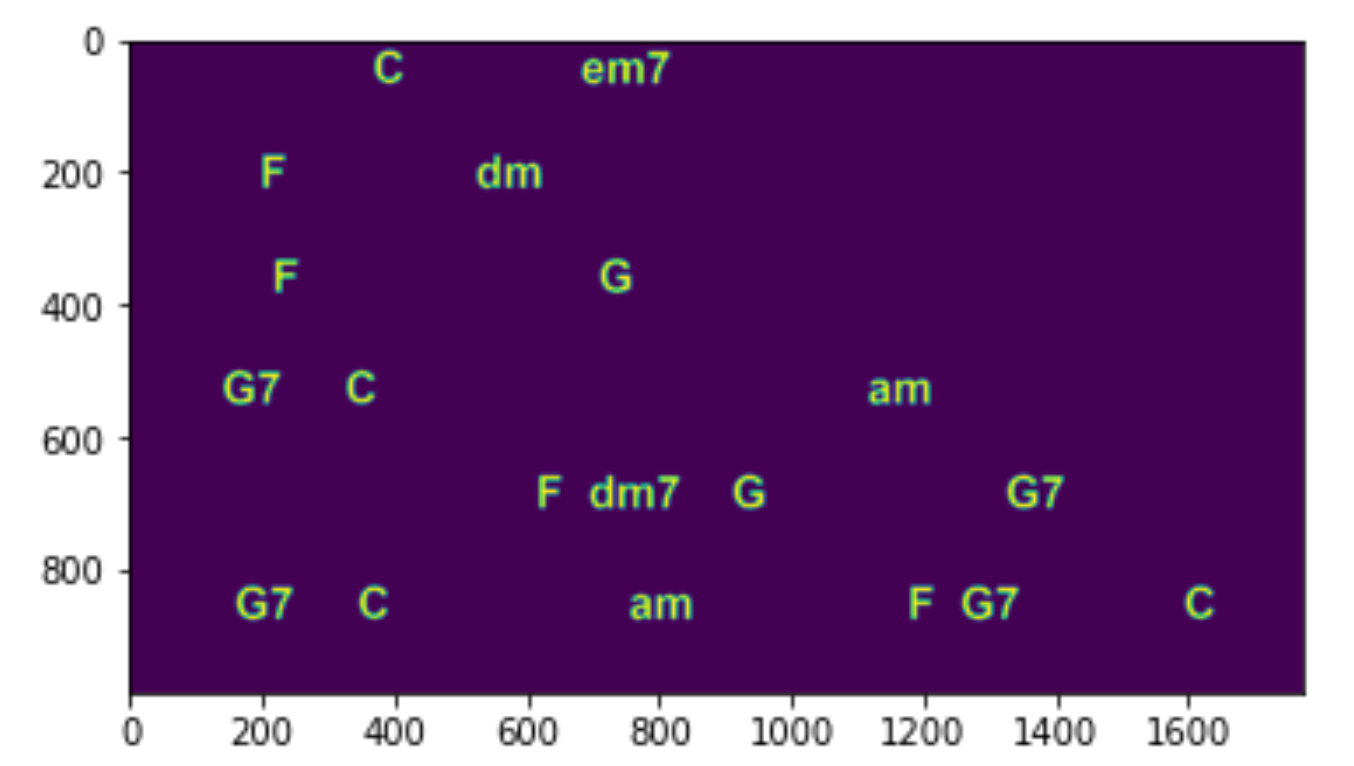
\includegraphics[width=\textwidth]{images/output_justchords.png}
	\caption{Kotta akkordjai}
	\label{fig:output2}
\end{figure}

\begin{figure}[h]
	\centering
	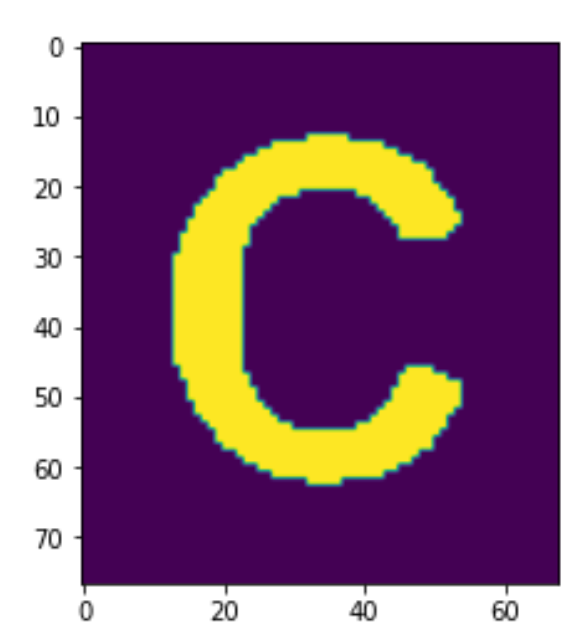
\includegraphics[scale=0.5]{images/output_single_character.png}
	\caption{A kotta egyik akkordja}
	\label{fig:output3}
\end{figure}

\begin{figure}[h]
	\centering
	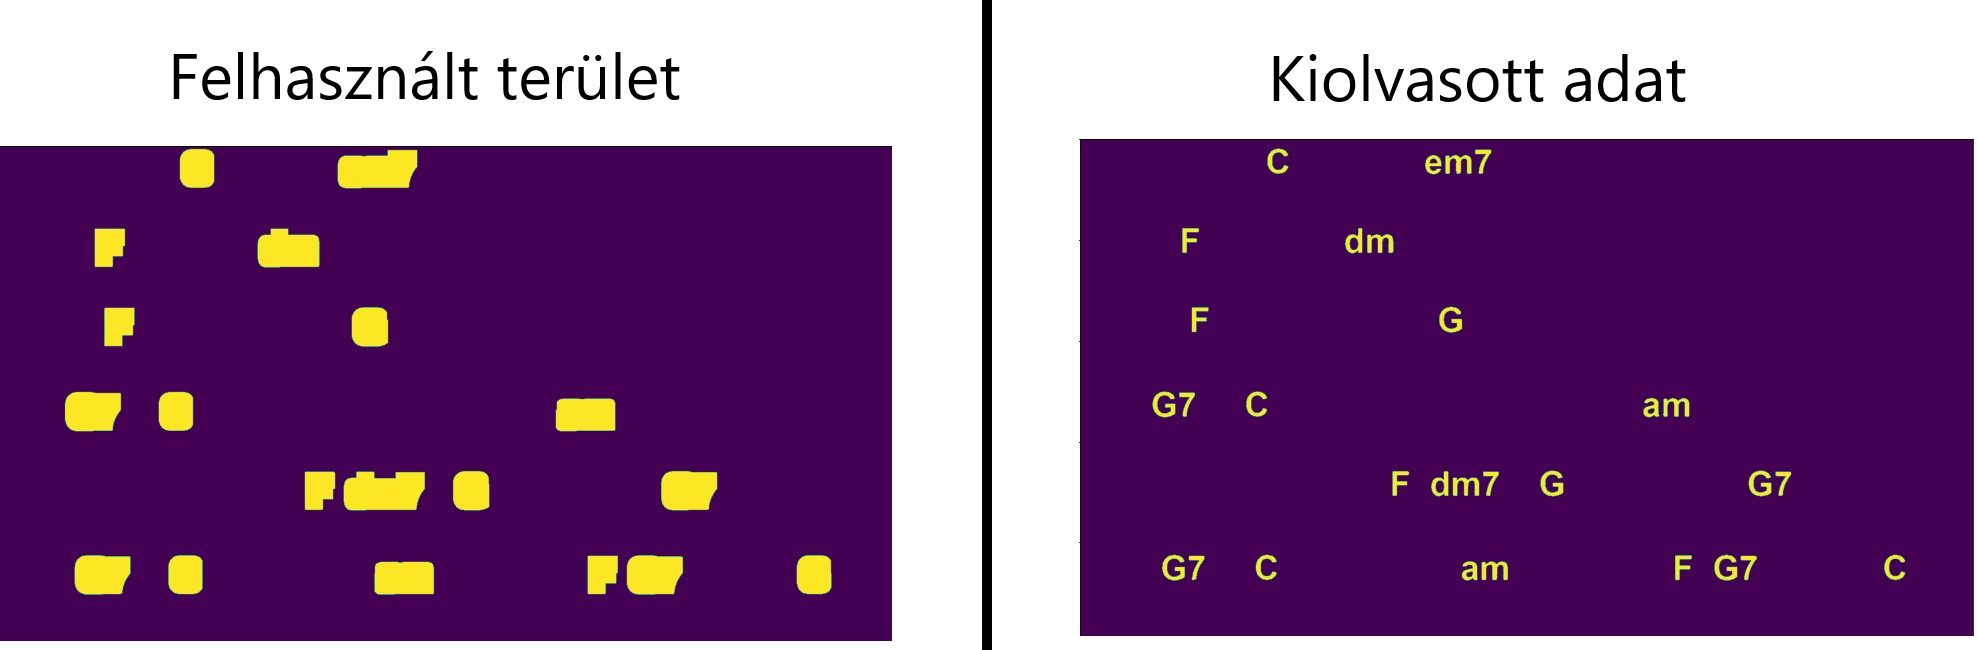
\includegraphics[width=\textwidth]{images/misc/chord_overlay.jpg}
	\caption{A terület és a kiolvasott adat, amit a program lát}
	\label{fig:output4}
\end{figure}

\Section{Lekérdezések kezelése}

Ebben a szekcióban lesz taglalva, hogy miként valósult meg az rdf egyes szerializációjának a betöltése és lekérdezése.

\SubSection{SPARQL}

Az RDF/XML féle szerializációval készítettem egy olyan programot ami betölti, majd feldolgozza az xml-t, hogy lekérdezéseket lehessen írni belőle. A következő lekérdezés kilistázza azokat az akkordokat, amelyek megtalálhatók a kottában.

\begin{python}
query_string_all_chord = """
    SELECT DISTINCT?o
    WHERE {
        ?s segment:note ?o .
        ?s ?p ?o .
    }
"""

q_res = g.query(query_string_all_chord)
for row in q_res:
    print(f"Akkord: {row.o}")
\end{python}
\begin{verbatim}
OUTPUT:
Akkord: C
Akkord: em7
Akkord: F
Akkord: dm
Akkord: F/G
Akkord: G
Akkord: G7
Akkord: am
Akkord: dm7
\end{verbatim}

Lekérdezhető az is, hogy milyen akkordhoz milyen szövegrész tartozik, vagy fordítva, ha szeretném megtudni azt, hogy egy szövegrészhez milyen akkord társul. Ehhez szükséges volna egy olyasfajta validáció, ami először végigpásztázza, hogy a kapott input az pontosan úgy megtalálható e a szerializált xml-ben, vagy sem.

\begin{python}
query_string_one_chord = '''
    SELECT ?s ?p ?o ?p1 ?o1
    WHERE {
        ?s ?p 'C' .
        ?s ?p ?o .
        ?s segment:text ?o1 .
        ?s ?p1 ?o1 .
    }
'''

q_res = g.query(query_string_one_chord)
for row in q_res:
    print(f"{row.o}\n {row.o1}")
\end{python}
\begin{verbatim}
OUTPUT:
C
 Tied a dicsőség, 
C
 mas, 
C
 mas, 
C
 mas!
\end{verbatim}
Kiegészítésként tenném hozzá még azt, hogy ez a lekérdezés használható abban az esetben is, ha több kotta áll rendelkezésre ugyanilyen sémával. A teendő annyi lenne vele, hogy egy rdf/xml sémában kellene letárolni a kották neveit valamint az ahhoz tartozó fontos információkat (pl.: hangnem, akkordok száma). Ha megjelenítésben gondolkozok, akkor az RDFa erre egy jó reprezentáció lenne, ahol ugyanis meg lehetne határozni azt, hogy egyes kották milyen forrás fájlt töltsenek be a megfelelő információkkal. Ez elősegíthet egy webes megjelenítést is, ahol a kották tárolása a felhőben lenne, és egyszerűen történhetne a lekérdezés SPARQL-lel.

\SubSection{Szimpla XML feldolgozása}

\begin{python}
tree = ET.parse(source='sheetparser.xml')

...

if child.tag == "segment":
	...
	
  if position_substring in line:
    occ = line.count(position_substring)
    ind_of_line = (line.replace(position_substring, '___', occ) + text)
      .find(position_substring)
    line.replace('___', position_substring, occ)
    line += text
  else:
    line += text
    ind_of_line = line.index(position_substring)
	            
     ...
     
  if segment_num.count(child.attrib['id']) > 0:
    ret += "\n"
    su += ret + line.replace(r'\n', "\n")
    ret, line = '', ''
    ind, notes = [], []
    count, sum_of_ind = 0, 0
\end{python}

A fenti programrészletben igyekeztem kiemelni a főbb pontokat, amiben ugyanis kiolvasom a már meglévő xml forrást és ezt felhasználva konzolra kiiratom a kottát akkordokkal pozícionálva. Ehhez megkeresi a program a segment tag-eket, ezekbe vannak letárolva az akkord, szöveg és pozíció adatok. 

Megkeresi a program, hogy egy adott sorban egyáltalán megtalálható e a pozíciós szöveg, majd megszámolja ennek az előfordulását. Ugyanis megtörténik az nagyon egyszerűen, hogy egy sorban többször is ismételhet ugyan az a pozíciós szöveg. Ez a pozíciós szöveg részét képezi az egész szövegnek, így nagyobb előfordulás miatt a programnak képesnek kell lennie ezt lekezelni. Helyettesítő string-et használva a program megjelöli az előfordulásokat, bepozícionálja az akkordot, majd visszahelyezi a szövegrészt.

Amit még érdemes megemlíteni, az az, mikor sortörés következik. Jelenleg a programban statikusan van letárolva egy tömbben azon szegmensek id-ja, amelyeknél sortörés történek, ez a \texttt{segment\_num} változóban van letárolva. Ezt, hogy dinamikusabb program legyen és több kottát is paraméterezve le tudjon kezelni, úgy lehet helyettesíteni, hogy lefuttatok egy külön ciklust, ami végigpásztázza a szegmenseket, és megkeresi azokat az előfordulásokat, ahol \texttt{\detokenize{'\n'}} található. Kiszedi a talált szegmens id-ját és letárolja ugyanúgy egy tömbben, vagyis ez pythonba listát jelent.

A konzolra kiiratott kottát (szöveges) a \ref{fig:output1}-es ábra mutatja

\begin{figure}[h]
	\centering
	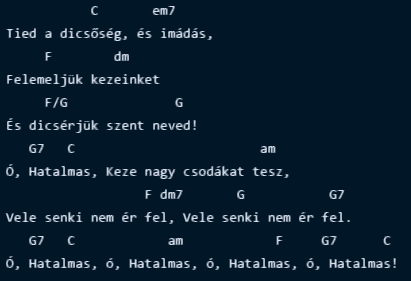
\includegraphics[scale=1]{images/output_tied.png}
	\caption{Az XML beolvasó program kimenete}
	\label{fig:output1}
\end{figure}
